\section{Entity Relationship Design}

\begin{landscape}
\thispagestyle{landscapefancy}
\centering
\IfFileExists{diagrams/generated/erd-overview.png}{%
\makebox[\linewidth][c]{%
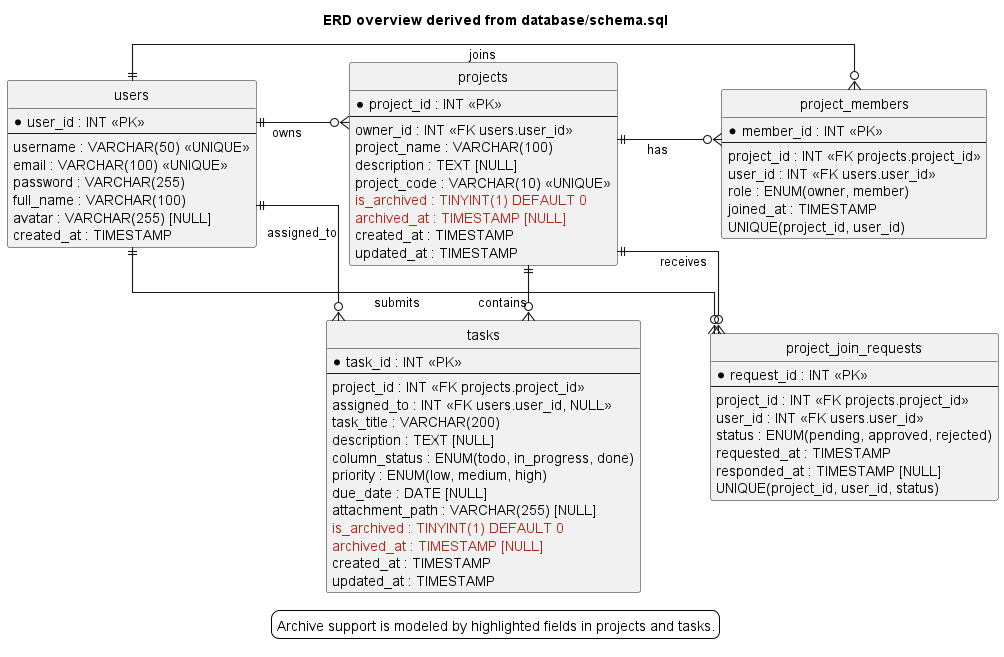
\includegraphics[width=0.90\paperheight,height=0.64\paperwidth,keepaspectratio]{diagrams/generated/erd-overview.png}%
}
}{%
\makebox[\linewidth][c]{%
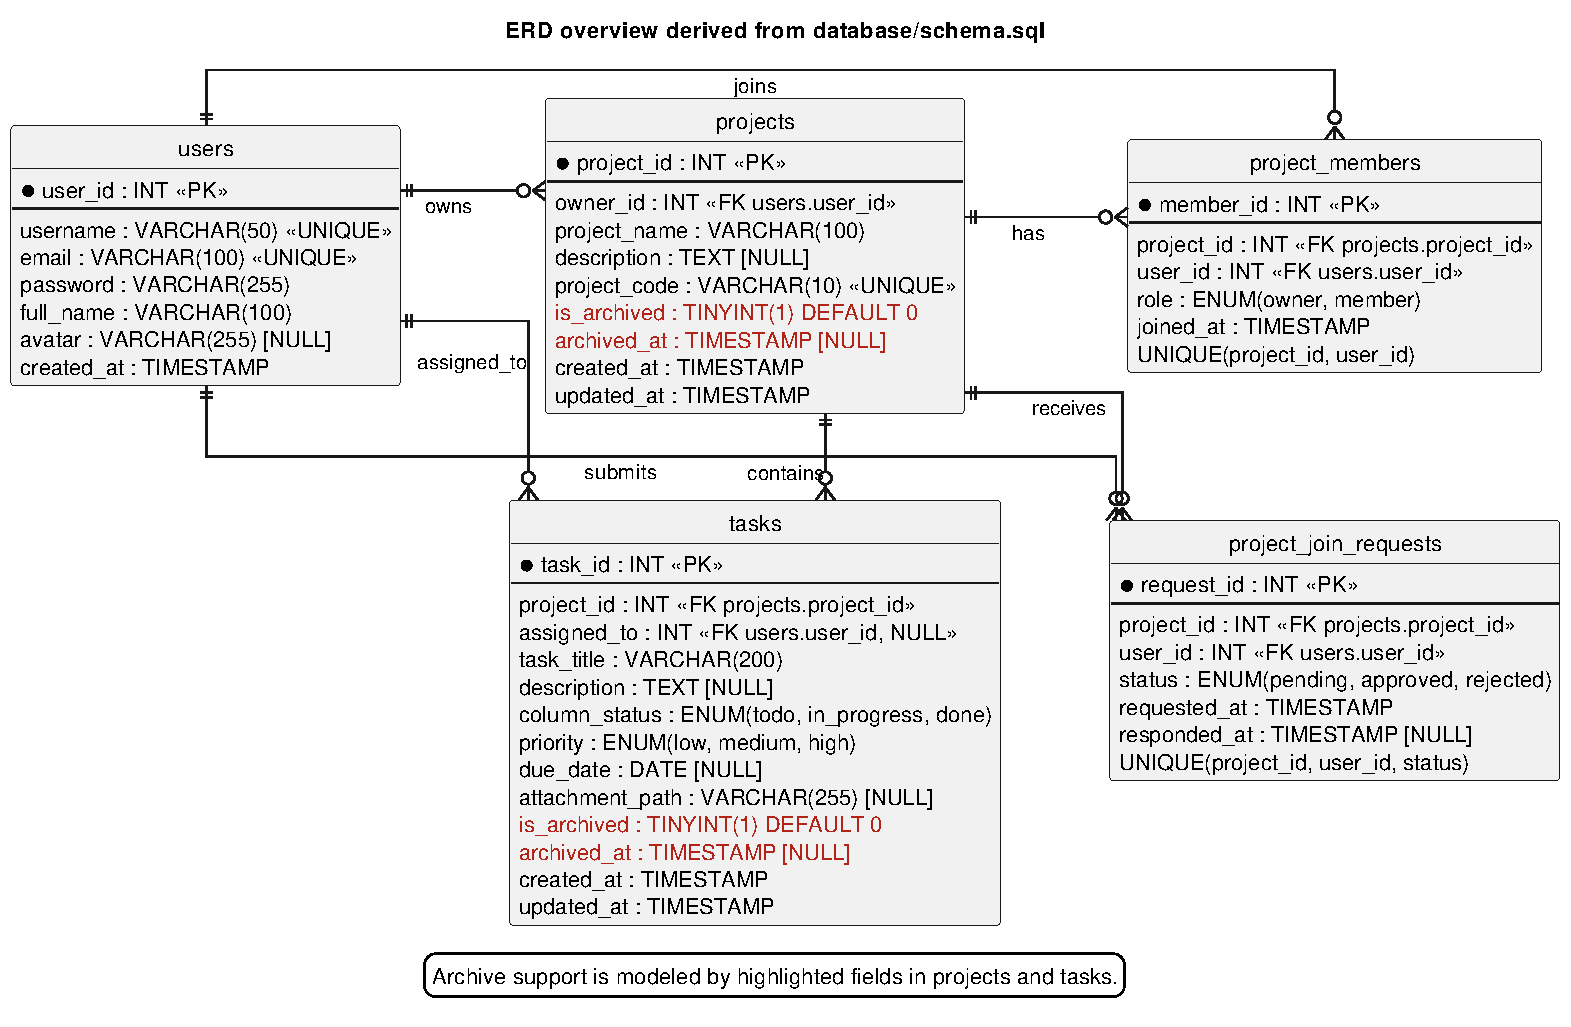
\includegraphics[width=0.90\paperheight,height=0.64\paperwidth,keepaspectratio]{diagrams/generated/erd-overview.pdf}%
}
}
\par\medskip
\captionof{figure}{ERD overview derived from \code{database/schema.sql} with archive fields}
\label{fig:erd-overview}
\end{landscape}
\clearpage


\subsection{Relationship Summary}

\begin{itemize}
    \item One user can own many projects (\code{projects.owner\_id}).
    \item One project can have many members via \code{project\_members}.
    \item One project can have many join requests via \code{project\_join\_requests}.
    \item One project can have many tasks.
    \item A task assignee may be \code{NULL} to represent unassigned work.
\end{itemize}

\subsection{Constraint Semantics}

\begin{itemize}
    \item \textbf{ON DELETE CASCADE}: deleting a project cascades to members, requests, and tasks.
    \item \textbf{ON DELETE SET NULL}: removing a user from assignment does not delete tasks; it clears \code{assigned\_to}.
    \item \textbf{UNIQUENESS}: duplicate project membership and duplicate pending requests are prevented by unique keys.
\end{itemize}
